% 定义文档类
\documentclass[12pt]{article} 

% 加入宏包
\usepackage{times}
\usepackage{epsfig}
\usepackage{graphicx}
\usepackage{amsmath}
\usepackage{amssymb}
\usepackage{authblk}  % 用来添加作者
\usepackage{cite}
\usepackage{float}
\usepackage{indentfirst}
\usepackage{subfigure}
\usepackage[colorlinks,
		linkcolor=green,
		anchorcolor=green,
		 citecolor=green]{hyperref}
\usepackage{geometry}


% 调整页边距
\geometry{a4paper,scale=0.7}
% 设置参考文献类型
\bibliographystyle{plain}

% 开始
\begin{document}
	
	% 标题
	\title{Research for better image captions:\\
		more accurate and diverse
	}

%	\author[1]{JiaCheng Zhang}
%	\affil[1]{School of Mathematics and Statistics, Central South University 
%	\authorcr Hunan, Changsha, China
%	\authorcr Jiachengzhang745@gmail.com}
	% 作者,单位,地址,和邮箱的另一种写法
	\author{Jiacheng Zhang \\
	School of Mathematics and Statistics, Central South University\\
	Hunan, Changsha, China\\
	% 让邮箱地址字体小一点
	{\tt\small Jiachengzhang745@gmail.com}
	}
	
	% 去掉默认显示编译时间
	\date{}
	
	\maketitle

	% 摘要
	\begin{abstract}
	Image captioning, which aims to automatically generate some natural language descriptions for an image, has attracted great research interest due to its wide application. This research proposal aims to research how to generate better, accurate and diverse image captions. Background of this research problem is presented first, then some previous work on generating accurate or diverse image captions is introduced. After that, three rough ideas about addressing this problem are proposed, 1) generate coarse-fine dynamic image captions based on scene graph, 2) develop an accuracy and diversity trade-off metric, and 3) image caption style transfer. The study of the challenges and problems around these rough ideas about image captioning will be the main focus of the follow-up research.
	\end{abstract}

	\section{Introduction}
	Image captioning, a task designed to automatically generate the appropriate natural language descriptions according to the content of an image, has recently received increasing attention. Not only because this task is very close to one of the core purposes of computer vision, scene comprehension, but also for its wide range of application, such as helping visually impaired people and assisting with text editing, etc.
	It is a research topic that combines computer vision and natural language processing, but definitely not a simple combination of them. In recent years, despite our remarkable achievements in the fields of computer vision and natural language processing, image captioning is still not well resolved. An important unsolved problem, for example, is how to produce accurate and diverse descriptions. As human beings, we can not only accurately describe the content of an image, but also use different methods to make the descriptions diversified. However, the current work of image captioning emphasizes either accuracy or diversity, and it is difficult to do both well, which leads to the descriptions we produce are either very simple, general, and rigid or have low accuracy.
	The purpose of this study is to focus on how to generate some accurate and diverse, even more interesting captions for an image. In this study, some rough ideas are proposed to solve this problem, and perfecting and realizing these ideas will be the focus of future research.
	
	\section{Literature Review}
	Image captioning has been studied for some time, and many models and approaches have been proposed. Among them, the methods based on deep learning have achieved very good results, which are also what we will focus on below.
	Because of the success of computer vision and natural language processing, people naturally thought of combining the two to solve this problem. In addition, as image captioning is a cross-modal problem, in which image to text conversion needs to be implemented, so, the encoder-decoder framework~\cite{cho2014learning} is widely used, in which the image is encoded to some features by the encoder, then the decoder is used to decode these features to the specific sentences. Vinyals, O ~\cite{vinyals2015show}proposed an end-to-end neural network which extracts visual features from input images using a Convolutional Neural Network (CNNs) and then generates a corresponding sentence from these features by RNN. This work provides a unified idea for the following works. Inspired by this work, a lot of related works following this paradigm have been proposed. The attention mechanism was first introduced by Xu, K. ~\cite{xu2015show} to guide the network to pay attention to specific positions in the image at each time step of the word generation. Following this, a lot of variants of attention mechanisms have been proposed. Chen, L ~\cite{chen2017sca} improved the current attention mechanism by combining spatial attention and channel-wise attention and proceed in a multi-layer form to get a better result. Peter Anderson, P ~\cite{anderson2018bottom} proposed a combined bottom-up and top-down attention mechanism that enables attention to the level of objects and salient image regions. ~\cite{pedersoli2017areas},~\cite{you2016image},~\cite{lu2017knowing} also proposed some other attention mechanisms like area attention, semantic attention, etc. These attention mechanisms significantly improved image caption generation. Besides, people also considered other factors that affect the quality of image caption generation. Wu, Q ~\cite{wu2016value} noted that the addition of high-level concepts could effectively improve the quality and accuracy of image caption generation, Yao, T  ~\cite{yao2017boosting} boosted the quality of the image caption by adding visual attributes. External information was also introduced to improve the result by Zhao, S.~\cite{zhao2019informative}. Of course, some new paradigms have also been proposed, such as Aneja, J. ~\cite{aneja2018convolutional} proposed a feed-forward convolutional (or CNN-based) approach to generate accurate image caption fast and reinforcement learning was also introduced by Rennie, S. J. ~\cite{rennie2017self} and has also achieved a good result.\par
	Most of the above methods just consider the accuracy of the generated description. However, the obsession with accuracy would make our descriptions simple, vague, and dull. For example, in order to improve the accuracy of the description, the network tends to use some common words or structures. So recently, how to generate diverse image captions has started to get a lot of attention. There is already some excellent work in this area. Instead of maximizing the likelihood of training samples, Dai, B ~\cite{dai2017towards} adopted conditional generative adversarial networks to jointly train a description generator and evaluator to generate more diverse descriptions. Wang, L ~\cite{wang2017diverse} similarly explored the application of conditional variational auto-encoders (CVAEs) to make diverse captions. Besides, Wang, Q. ~\cite{wang2017diverse} developed a new metric for evaluating the diversity of the caption set based on SVD. These methods have been proposed to generate diverse captions, but most of them are less accurate, which cannot do the both well.
	There is also some excellent work on how to produce accurate and diverse descriptions. For example, Liu, L. ~\cite{liu2019generating} generated diverse and descriptive image captions by using visual paraphrases which were the different sentences describing the same image selected from the dataset, instead of using beam search, Deshpande, A. ~\cite{deshpande2019fast} used part-of-speech (POS) as the guidance to get diverse and accurate image captions. However, there is still much space for improvement.
	
	\section{Purpose of study}
	Image captioning has a wide range of applications, which makes it very valuable to study. Although the descriptions we now produce have achieved very good accuracy on many evaluation metrics, just as each of us speaks differently, we are not satisfied with generating the right descriptions for an image. We hope that the generated descriptions can be diversified to meet different requirements. For example, sometimes we may just want to know what are the objects in the image and how their positional relationship is, but sometimes we may need more details about the content of the image, such as the characteristics and status of each object inside, and for another example, in the auxiliary text editing, sometimes we may need a length limited description of the image, and sometimes we may want the description to be not only accurate, but also as beautiful as possible. So, knowing how to produce accurate and diverse picture descriptions is very important, and that is also the main purpose of this study. It's must be a creative and joyful journey for me if I could contribute to this unsolved challenging problem a little.
	
	\section{Research question}
	The main problem of this study is about how to generate more accurate and diverse image captions for an image. Some rough ideas are presented below.
	\subsection{Coarse-Fine dynamic image captions based on scene graph}
	Image captioning aims to automatically generate fluent natural language to describes the salient content of an image. This includes objects in the picture, their attributes, and the relationships between objects. In fact, this corresponds to the structure and composition of a sentences. In simple terms, entities in pictures correspond to nouns in sentences, attributes of entities correspond to adjectives in sentences, and relationships correspond to verbs, etc. So, image caption is a natural description of the scene posed in the image. How do we describe a scene? Imagine giving you a picture and asking you to describe what's inside, how would you do that? Generally speaking, our processing will be a gradual process. For example, at the beginning, we might just see what are the objects in the image? And then observe what they are doing? Next, we will add some details to them, such as what the entities look like and what their state is. It's like telling a story to children with a storybook, first to outline, and then to keep adding details. In addition, just as we tell a story, the same story will be explained differently from the perspectives of different roles, so we can also make different interpretations of the same scene from the perspective of different objects. In fact, the process mentioned above actually reflects the different diversity of the descriptions 1) different semantics, different level of detail of descriptions, and usually affect the length of descriptions 2) different syntax, structure, different sequence of descriptions.\par
	Due to the lack of relevant knowledge, I can only try to give a general description of the idea mentioned above from the perspective of implementation. In general, a given training data is a set of images and their captions, when training, first, we use a grammar parser to parse the description of the image and break it into different components of the sentence, such as nouns and adjectives, etc. And then, based on the sentence structure and syntax, these components are constructed into a graph representing the meaning of the sentence. After that, we can follow the work of Fang, H. ~\cite{fang2015captions}, we train some words or concepts detectors using weakly-supervised approach of Multiple Instance Learning, which are mainly to detect the entities of the image. After that, we can take the graph built before as the supervisory signal, and take the words detectors as the foundation to train a network which can build a scene graph from an image according its content. In the scene graph, the nodes represent objects and the edges are relations between pairs of objects. And then we can take this scene graph as input of the following LSTM or some other language models to generate the final descriptions. But in order to get diverse captions, we can apply attention mechanism on the graph, we can develop a visual attribute prediction model like ~\cite{you2016image}, then, if a node representing an entity of the image in the graph is paid special attention, we can detect its corresponding attributes for the entity in the image. After that, we add these attributes to the following networks to get more detail description of the objects. The way that the following LSTM parse the graph also matters, for example, the beginning node is generally used as the main body of the sentence, the path and direction of parsing represent the content and the words sequence in the sentence. In this way, we can describe the image just like human beings, for example, we can first focus on the main parts, generate a very simple description, and then notice a specific object, describe the properties of that object in the sentence, and we can also adjust the structure of the sentence we describe. See the Figures below for an overview of the process.
	
	\begin{figure}[H]	
		\centering
		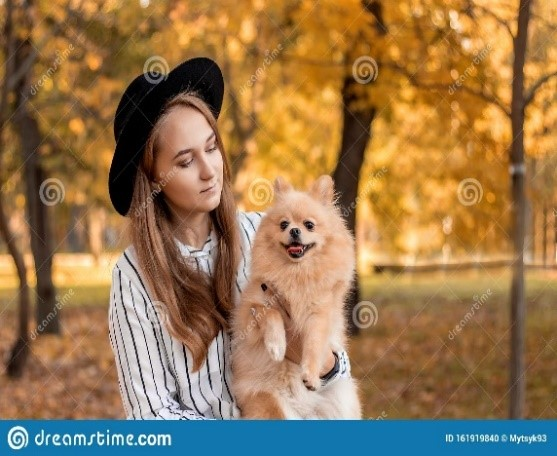
\includegraphics[trim={0 0.5cm 0 0},clip]{images/Figure1.jpg}
		\caption{Input image}
		\label{fig1}
	\end{figure}
	\textbf{Ground truth}: A blonde woman in a black and white striped dress and a black hat was standing in the forest holding a small yellow dog.
	\begin{figure}[H]	
		\centering
		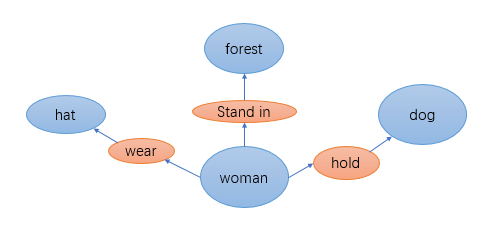
\includegraphics[]{images/Figure2.png}
		\caption{Scene graph based on the image}
		\label{fig2}
	\end{figure}

	\begin{figure}[H]
		\centering
		\subfigure[]{
			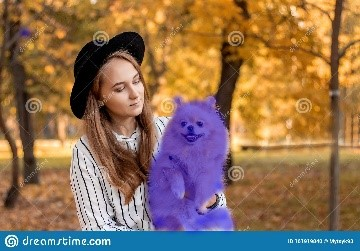
\includegraphics[scale=0.8,trim={0 0.5cm 0 0},clip]{images/Figure3-1.jpg} 
		}
		\subfigure[]{
			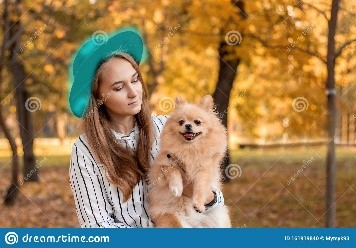
\includegraphics[scale=0.8,trim={0 0.5cm 0 0},clip]{images/Figure3-2.jpg}
		}
		\subfigure[]{
			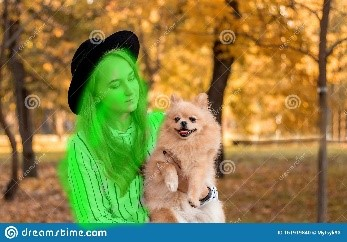
\includegraphics[scale=0.8,trim={0 0.5cm 0 0},clip]{images/Figure3-3.jpg}}
		\caption{Pay attention to different entities to get their attributes}
		\label{fig3}
	\end{figure}
	
		\begin{figure}[H]
		\centering
		\subfigure[]{
			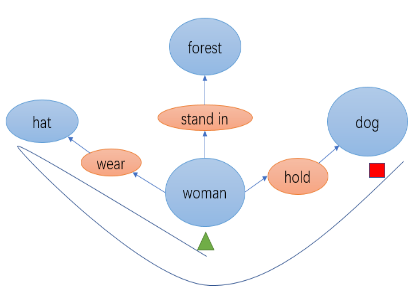
\includegraphics[scale=0.8]{images/Figure4-1.png} 
		}
		\subfigure[]{
			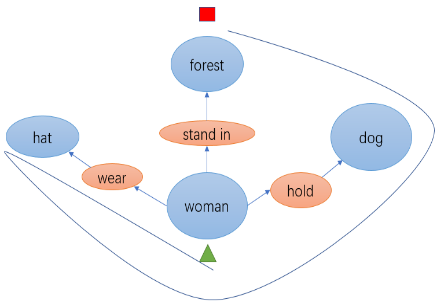
\includegraphics[scale=0.8]{images/Figure4-2.png}
		}
		\subfigure[]{
			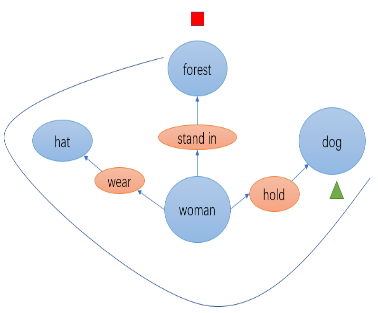
\includegraphics[scale=0.8]{images/Figure4-3.png}}
		\caption{Different ways to parse the scene graph (green: start, red: end)}
		\label{fig4}
	\end{figure}

	\textbf{Generated captions:}  \\
	(1)	A woman holding a dog.  							             \hfill (coarse)  \\
	(2)	A woman holding a dog standing in the forest. 		 	    \hfill (include the forest) \\
	(3)	A woman holding a yellow dog stand in the forest.		\hfill  	(add details of dog)  \\
	(4)	A woman wearing a hat holding a yellow dog standing in the forest.                \\
	(5)	A woman wearing a black hat holding a yellow dog standing in the forest.	\hfill (fine)  \\
	(6)	A dog hold by a woman standing in the forest.     \hfill 	    (change structure)         \\
	…  \par
	The above is just a simple idea, there are still many problems in it. For example, how to construct the scene graph, maybe the method mentioned above doesn’t work, how to realize the alignment of words with image entities, how to implement attributes detection, and how to parse the constructed scene graph? These are all challenging problems that need to be solved in future research.
	
	\subsection{Accuracy and diversity trade-off metric}
	One of the reasons why image captioning is so challenging is that it is very difficult to find a suitable evaluation metric to measure the results. At present, the most commonly used evaluation metrics are mainly BLEU, METEOR, ROUGE, CIDEr, SPICE etc. There are some differences between them in the evaluation criteria. BLEU, METEOR, ROUGE, CIDEr are based on calculating the words overlap between generated and the reference caption, and SPICE computes the similarity of the scene graph built by the generated caption and the reference caption. However, none of these approaches strike a good balance between accuracy and diversity. For example, the metrics based on computing words overlap fail to correlate well with human judgments for weakness to capture the meaning of a sentence, while SPICE is so sensitive to the semantic that ignore the diversity of sentences. As a result, methods based on these evaluation metrics cannot achieve good results, such as CVAE, CGAN model. Thus, we urgently need an evaluation metric that can balance accuracy and diversity well. \par
	For accuracy evaluation, the existing methods either cannot reflect the semantic structure well, or are too complex, and they can be comprehensively improved. For example, for CIDEr, simply counting the number of overlapping words may not accurately reflect the semantic structure. For example, the network can use synonyms or synonyms to express the same or similar meaning with a real caption, and such result usually cannot get a high accuracy score. Therefore, we can map the description to a suitable semantic space first, and then some criterion of accuracy is used in the semantic space, like calculating the distance of vectors in the semantic space. In this way, we can get a better accuracy evaluation method.  \par
	Generally speaking, the diversity of descriptions is mainly reflected in three aspects: different words, different grammatical structures, and different semantics. Most of the current work on diversity focuses on semantic differences, such as ~\cite{wang2019describing}, use LSA to map the generated caption to the topic space, and apply the SVD to decompose the similarity matrix and measure the diversity of generated captions by the distribution of eigenvalues in the topic space, where topic actually corresponds to the semantics. However, the same meaning can be expressed in different ways, such as using some synonyms or synonyms, or using different sentence structures. How to measure these two diversities? Here are some of my thoughts: for the former, by using word embedding network, we can first search for each word in the embedded space through the nearest neighbor to find out k words which are the synonym with the word. And then, when we get the captions, we can take the frequency of synonyms in sentences as the ability of the network to use synonyms. The latter may be a little more difficult, because the grammatical structure may be the most difficult in a language, but there are still some things we can try. Referring to the current work of natural language processing, we can parse a sentence into a syntax tree according to its syntax. The structure of this tree actually represents the grammatical structure of the whole sentence. Finally, by calculating the similarity between different grammatical trees, for example, using the graph neural network to represent the grammar tree and to get the distance of them, we can measure the diversity of different captions in terms of syntax structure.  \par
	After we can measure accuracy and diversity well, an accuracy-diversity trade-off metric can be obtained by weight sum or other method like using ensemble matrix ~\cite{wang2020diversity}. Once we have this evaluation metric, we can evaluate the accuracy and diversity of the generated image captions, and then, like ~\cite{rennie2017self}, we can apply the reinforcement learning to directly optimize this metric and force the network to generate accurate and diverse image captions.
	\subsection{More interesting: image caption style transfer}
	Imagine if you were a teacher, and you gave your classmates an assignment to look at an image and write, what kind of results would you most like to see? First of all, the most important thing is that students' compositions should be based on the image and reflect the real content of it. What else? Different students should have different writing styles, just like we speak, and of course, we want students to write in different styles that reflect their personalities. So, another diversity of descriptions, in my opinion, is the diversity of description styles.  \par
	
	
	\begin{figure}[H]
		
		\begin{minipage}{0.32\linewidth}
			\vspace{3pt}
			%这个图片路径替换成你的图片路径即可使用
			\centerline{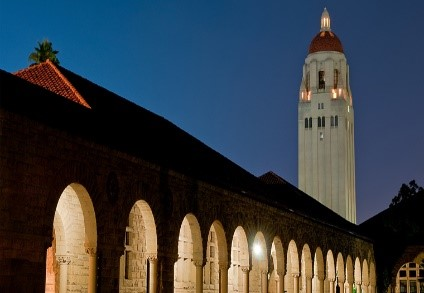
\includegraphics[width=\textwidth]{images/Figure5-1.jpg}}
			% 加入对这列的图片说明
			\centerline{orignal}
		\end{minipage}
		\begin{minipage}{0.32\linewidth}
			\vspace{3pt}
			\centerline{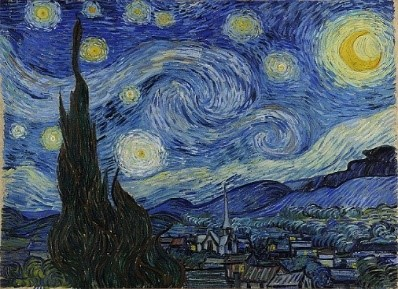
\includegraphics[width=\textwidth]{images/Figure5-2.jpg}}
			
			\centerline{target}
		\end{minipage}
		\begin{minipage}{0.32\linewidth}
			\vspace{3pt}
			\centerline{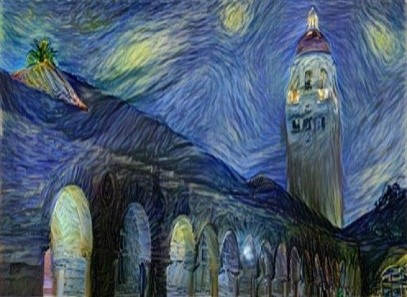
\includegraphics[width=\textwidth]{images/Figure5-3.jpg}}
			
			\centerline{result}
		\end{minipage}
		
		\caption{Neural Style Transfer}
		\label{fig5}
	\end{figure}
	
	
	In fact, just like neural style transfer, which makes one image have the same painting style as another image as shown in Figure.5, we can also think about the style transfer of the image caption. At present, we have a lot of corpus, which includes a lot of famous literary works, which to a certain extent, reflect the author's writing style, such as the collection of Shakespeare's works, Hemingway's works and so on. So, we can do something more interesting, transfer the writing style of these famous authors to our descriptions of the images, and then we can see, what will these authors think when they are showed these images, how would they describe what they see. In this way, we can generate very interesting descriptions. For example, for an image, the descriptions of Shakespeare's style may be brilliant, while the descriptions of Nietzsche's style are likely to be critical. \par
	From the perspective of implementation, the main difficulty in the current text style transfer is the lack of parallel style transfer training samples, so, we can refer to the work of ~\cite{luo2019dual} to use meta-reinforcement learning and unsupervised learning to directly model the mapping relationship from one text style to another text style, thereby obtaining a text style converter. However, this method is actually two-stage, first generating the original description text for the picture, and then using this text style converter to convert it to another style. This might be time-consuming. We can try to integrate these two parts together, learn the content in the image and the style of reference text at the same time during the training, and generate the corresponding style of image descriptions. However, this may require further research on network structure, learning methods and other aspects.  \par
	
		\begin{figure}[H]	
		\centering
		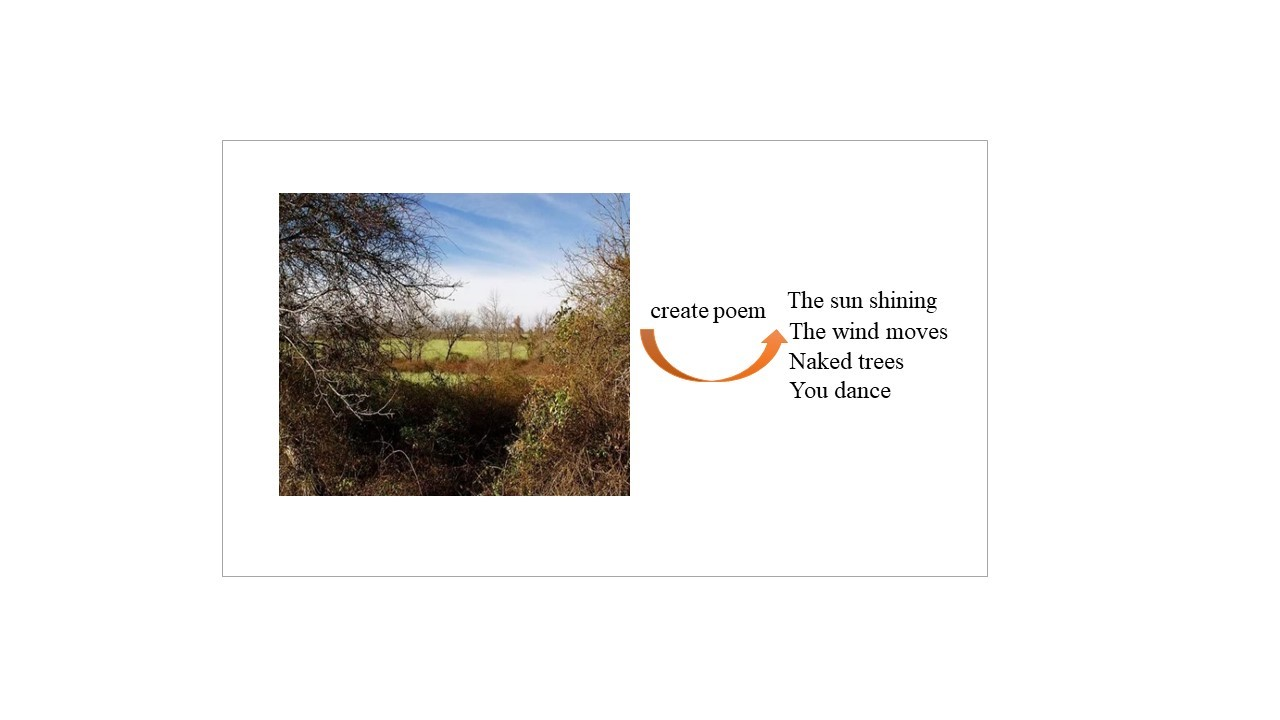
\includegraphics[scale = 0.4,trim={6cm 5cm 9cm 5cm},clip]{images/Figure6.jpg}
		\caption{The input image and poem created by the network.}
		\label{fig1}
		\end{figure}
	Actually, Liu, B. ~\cite{liu2018beyond} has already tried to use the methods of multi-adversarial training via policy gradient to teach the network to create poems about the content of images by Generative Adversarial Network. Here, poetry is actually a particular descriptive style. Figure.6 shows the poem created by the network based on the input image, which is really full of artistry. So, this is a very interesting direction that is worth exploring.
	
	\section{Methodology and research plan}
	\subsection{Research method}
	Combination of theoretical study and practical verification. For each problem, it is necessary not only to analyze the problem theoretically and propose a solution based on related knowledge, but also to verify the feasibility of the proposed method in practice and analyze some characteristics of the method itself through experiments. Specifically, the research process can be divided into four stages, first investigate the feature of the specific problem and the current work, after that, analyze the problem based on the current theoretical knowledge and propose some ideas, and then design a practical experimental scheme to validate these ideas, finally, carry out experiment to check the design and make some adjustment according to the result of the experiment until the final conclusion is reached.
	
	\subsection{Research Plan}
	After putting forward some preliminary ideas above, In order to better carry out scientific research and realize the above ideas in the future research, some research plans have been formulated.
	\renewcommand{\labelenumi}{\Roman{enumi}}
	\begin{enumerate}
		\item Prepare required knowledge and theory about this filed  \par
			At the beginning, relevant theories and fundamental knowledge about this field are required, including linear algebra, probability and statics, machine learning, computer vision etc. Another task is to learn some specific knowledge about the intersection of computer vision and natural language process. Besides, in order to gain some intuitions and insight about image captioning and keep up with the pace of research in this field, literature review will be updated every month.
		\item Research for accurate image captions  \par
			Based on the basic requirement of image captioning, investigate the way of generating accurate image captions. Firstly, review some good methods proposed by other scholars, and then analyze the advantages and disadvantages of these methods, obtain inspiration from them and propose some new ideas to generate image captions that are more relevant to human annotations, and finally, do some experiments to validate and adjust.
		\item Research for diverse image captions \par
			According to the characteristics of image captioning, study how to generate more diversified image captions from different perspectives, such as evaluation metrics, model structure, and sentence generation methods and so on. Besides, think about how to apply some other effective methods to solve this problem, such as reinforcement learning, graph neural network, etc. And always pay attention to some of the latest methods to solve the problem, so as to get some inspiration.
		\item Combine accuracy and diversity to make better image captions \par
			Surrounding these rough ideas mentioned above, study the details of each part and propose effective solutions to the existing problems. Then the experimental scheme is designed to verify the above ideas and continuously improve the results and finally establish a new baseline of generating better descriptions of an image.
	\end{enumerate}
	 
	
	
	\section{Conclusion}
	Image captioning as an intersectional field of computer vision and natural language processing is full of challenges and huge application potential. However, this problem has not been well resolved yet. The purpose of this research is to find out a better way to automatically generate more accurate and diverse descriptions for an image which are similar to human annotations. In this proposal, we review some previous work on this problem first, both on accuracy and diversity, and then some rough ideas about making better image captions are presented, even though these ideas may still have many theoretical and implementation problems. Finally, in order to better carry out the research, a basic research method has been proposed and a series of research plans have been formulated.  \par
	I hope I could have the opportunity to carry out my research according to this proposal to realize the ideas mentioned above and make some contributions to solve this problem.
	
\bibliography{ref.bib}

\end{document}